%%%%%%%%%%%%%%%%%%%%%%%%%%%%%%%%%%%%
% Slide options
%%%%%%%%%%%%%%%%%%%%%%%%%%%%%%%%%%%%

% Option 1: Slides with solutions

\documentclass[slidestop,compress,mathserif]{beamer}
\newcommand{\soln}[1]{\textit{#1}}
\newcommand{\solnGr}[1]{#1}

% Option 2: Handouts without solutions

%\documentclass[11pt,containsverbatim,handout]{beamer}
%\usepackage{pgfpages}
%\pgfpagesuselayout{4 on 1}[letterpaper,landscape,border shrink=5mm]
%\newcommand{\soln}[1]{ }
%\newcommand{\solnGr}{ }

%%%%%%%%%%%%%%%%%%%%%%%%%%%%%%%%%%%%
% Style
%%%%%%%%%%%%%%%%%%%%%%%%%%%%%%%%%%%%
\def\chp1@path{../../Chp 1}
\input{../../lec_style.tex}


%%%%%%%%%%%%%%%%%%%%%%%%%%%%%%%%%%%%
% Preamble
%%%%%%%%%%%%%%%%%%%%%%%%%%%%%%%%%%%%

\title[Lecture 2]{MA213: Lecture 2}
\subtitle{Module 1: Exploratory Data Analysis and Study Design}
\author{OpenIntro Statistics, 4th Edition}
\institute{$\:$ \\ {\footnotesize Based on slides developed by Mine \c{C}etinkaya-Rundel of OpenIntro. \\
The slides may be copied, edited, and/or shared via the \webLink{http://creativecommons.org/licenses/by-sa/3.0/us/}{CC BY-SA license.} \\
Some images may be included under fair use guidelines (educational purposes).}}
\date{}

%%%%%%%%%%%%%%%%%%%%%%%%%%%%%%%%%%%%
% Begin document
%%%%%%%%%%%%%%%%%%%%%%%%%%%%%%%%%%%%

\begin{document}


%%%%%%%%%%%%%%%%%%%%%%%%%%%%%%%%%%%%
% Title page
%%%%%%%%%%%%%%%%%%%%%%%%%%%%%%%%%%%%

{
\addtocounter{framenumber}{-1} 
{\removepagenumbers 
\usebackgroundtemplate{\includegraphics[width=\paperwidth]{../../OpenIntro_Grid_4_3-01.jpg}}
\begin{frame}

\hfill \includegraphics[width=20mm]{../../oiLogo_highres}

\titlepage

\end{frame}
}
}


%%%%%%%%%%%%%%%%%%%%%%%%%%%%%%%%%%%%
% Recap/Agenda 
%%%%%%%%%%%%%%%%%%%%%%%%%%%%%%%%%%%%
% TODO better formatting
\begin{frame}
    \frametitle{Module 1: Exploratory Data Analysis and Study Design}
    \begin{itemize}
        \item \hl{Previously: }Course introduction, survey
        \item \hl{This time: }Introduction to data (Chapter 1)
        \item \hl{Reading: }Chapter 2 for next time
        \item \hl{Deadlines/Announcements: }HW 1.1 due next Monday
    \end{itemize}
    
\end{frame}
    

%%%%%%%%%%%%%%%%%%%%%%%%%%%%%%%%%%%%
% Sections
%%%%%%%%%%%%%%%%%%%%%%%%%%%%%%%%%%%%

\section{Jumping in: Data basics}

%%%%%%%%%%%%%%%%%%%%%%%%%%%%%%%%%%%%

\subsection{Observations and variables}

\begin{frame}
\frametitle{Classroom survey}

A survey was conducted on students in an introductory statistics course. Below are a few of the questions on the survey, and the corresponding variables the data from the responses were stored in:

\begin{itemize}
\item \var{gender}: What is your gender? 
\item \var{intro\_extra}: Do you consider yourself introverted or extraverted? 
\item \var{sleep}: How many hours do you sleep at night, on average?
\item \var{bedtime}: What time do you usually go to bed?
\item \var{countries}: How many countries have you visited?
\end{itemize}

\end{frame}

%%%%%%%%%%%%%%%%%%%%%%%%%%%%%%%%%%%%

\begin{frame}
\frametitle{Data matrix}

Data collected on students in a statistics class on a variety of variables:

\begin{center}
\begin{tabular}{l cccc l}
		& \hl{variable} \\
		& \hl{$\downarrow$}	 \\
\cline{1-5}
Stu.	&	\var{gender}	&	\var{intro\_extra} & $\cdots$ & \var{countries} \\
\cline{1-5}
1 & male   & extravert  & $\cdots$  & 13 \\ 
2 & female & extravert  & $\cdots$  & 7 \\ 
3 & female & introvert  & $\cdots$  & 1 & \hl{$\leftarrow$}  \\ 
4 & female & extravert  & $\cdots$  & 5 & \hl{observation} \\
$\vdots$	 &	$\vdots$	&	$\vdots$  &	$\vdots$ &	$\vdots$ \\
86	& male & extravert  & $\cdots$  & 9 \\
\cline{1-5}
\end{tabular}
\end{center}

\end{frame}

%%%%%%%%%%%%%%%%%%%%%%%%%%%%%%%%%%%%

\subsection{Types of variables}

\begin{frame}
\frametitle{Types of variables}

\begin{center}
\includegraphics[width=0.9\textwidth]{\chp1@path/1-2_data_basics/figures/variables/variables}
\end{center}

\end{frame}

%%%%%%%%%%%%%%%%%%%%%%%%%%%%%%%%%%%

\begin{frame}
\frametitle{Types of variables (cont.)}

\begin{center}
{\footnotesize
\begin{tabular}{c ccc cc}
  \hline
 & \var{gender} & \var{sleep} & \var{bedtime} & \var{countries}  \\
  \hline
1 & male & 5 & 12-2 & 13  \\ 
  2 & female & 7 & 10-12 & 7  \\ 
  3 & female & 5.5 & 12-2 & 1  \\ 
  4 & female & 7 & 12-2 &   \\ 
  5 & female & 3 & 12-2 & 1  \\ 
  6 & female & 3 & 12-2 & 9  \\ 
  \hline
\end{tabular}
}
\end{center}

\begin{itemize}
\item \var{gender}: \pause \soln{\only<2->{categorical}} \pause
\item \var{sleep}: \pause \soln{\only<4->{numerical, continuous}} \pause
\item \var{bedtime}: \pause \soln{\only<6->{categorical, ordinal}} \pause
\item \var{countries}: \pause \soln{\only<8->{numerical, discrete}} \pause
\end{itemize}

\end{frame}

%%%%%%%%%%%%%%%%%%%%%%%%%%%%%%%%%%%

%%%%%%%%%%%%%%%%%%%%%%%%%%%%%%%%%%%%
\section{R Demo: Loading and Visualizing Data}
%%%%%%%%%%%%%%%%%%%%%%%%%%%%%%%%%%%%%

%%%%%%%%%%%%%%%%%%%%%%%%%%%%%%%%%%%

\subsection{Relationships among variables}

%%%%%%%%%%%%%%%%%%%%%%%%%%%%%%%%%%%

\begin{frame}
\frametitle{Relationships among variables}

\dq{Does there appear to be a relationship between GPA and number of hours students study per week?}

\begin{center}
\includegraphics[width=0.7\textwidth]{\chp1@path/1-2_data_basics/figures/gpa_study_hours/gpa_study_hours}
\end{center}

\pause

\dq{Can you spot anything unusual about any of the data points?}

\soln{\pause{There is one student with GPA $>$ 4.0, this is likely a data error.}}

\end{frame}

%%%%%%%%%%%%%%%%%%%%%%%%%%%%%%%%%%%

\subsection{Explanatory and response variables}

%%%%%%%%%%%%%%%%%%%%%%%%%%%%%%%%%%%

\begin{frame}
\frametitle{Explanatory and response variables}

\begin{itemize}

\item To identify the explanatory variable in a pair of variables, identify which of the two is suspected of affecting the other:

\begin{center}
explanatory variable $\xrightarrow{might~affect}$response variable
\end{center}

\item Labeling variables as explanatory and response does not guarantee the relationship between the two is actually causal, even if there is an association identified between the two variables. We use these labels only to keep track of which variable we suspect affects the other.

\end{itemize}

\end{frame}

%%%%%%%%%%%%%%%%%%%%%%%%%%%%%%%%%%%

\subsection{Introducing observational studies and experiments}

%%%%%%%%%%%%%%%%%%%%%%%%%%%%%%%%%%%

\begin{frame}
\frametitle{Two primary types of data collection}

\begin{itemize}

\item \hl{Observational studies:} Collect data in a way that does not directly interfere with how the data arise (e.g. surveys).
\begin{itemize}
\item Can provide evidence of a naturally occurring association between variables, but they cannot by themselves show a causal connection.
\end{itemize}

\pause

\item \hl{Experiment:} Researchers randomly assign subjects to various treatments in order to establish causal connections between the explanatory and response variables.


\end{itemize}

\end{frame}

%%%%%%%%%%%%%%%%%%%%%%%%%%%%%%%%%%%

\begin{frame}
\frametitle{Association vs. causation}

\begin{itemize}

\item When two variables show some connection with one another, they are called \hl{associated} variables.
\begin{itemize}
\item Associated variables can also be called \hl{dependent} variables and vice-versa.
\end{itemize}

\item If two variables are not associated, i.e. there is no evident connection between the two, then they are said to be \hl{independent}.

\item In general, association does not imply causation, and causation can only be inferred from a randomized experiment.

\end{itemize}

\begin{center}
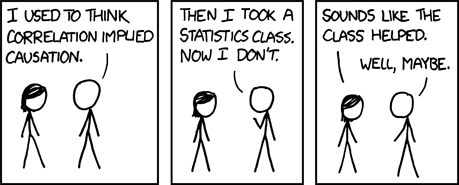
\includegraphics[width=0.55\textwidth]{\chp1@path/1-2_data_basics/figures/xkcd_correlation} \\
{\tiny \webURL{http://xkcd.com/552/}}
\end{center}

\end{frame}

%%%%%%%%%%%%%%%%%%%%%%%%%%%%%%%%%%%%

%%%%%%%%%%%%%%%%%%%%%%%%%%%%%%%%%%%

\section{Sampling principles and strategies}

%%%%%%%%%%%%%%%%%%%%%%%%%%%%%%%%%%%%

\subsection{Populations and samples}

%%%%%%%%%%%%%%%%%%%%%%%%%%%%%%%%%%%%

\begin{frame}
	\frametitle{Populations and samples}

	\twocol{0.4}{0.6}{
	\begin{center}
	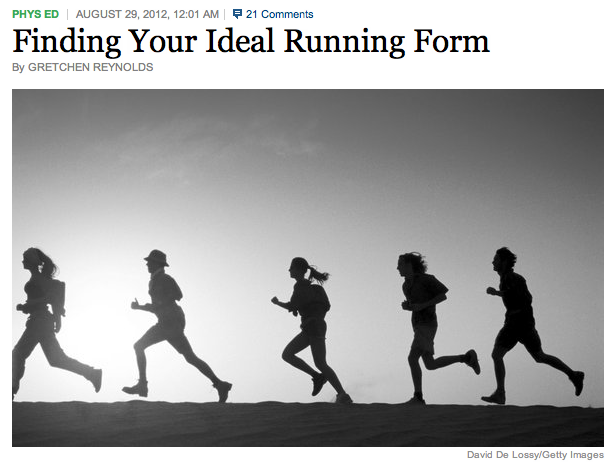
\includegraphics[width=\textwidth]{\chp1@path/1-3_sampling_principles_strategies/figures/running.png}
	\end{center}
	\vspace{-0.5cm}
	{\tiny \webURL{http://well.blogs.nytimes.com/2012/08/29/finding-your-ideal-running-form}}
	}
	{
	\hl{Research question:} Can people become better, more efficient runners on their own, merely by running? \\

	\pause 

	\hl{Population of interest:} \soln{\pause All people}\\
	\hl{Population parameter of interest:} \soln{\pause Average change in running pace after 10 weeks}
	}
	\pause 
	$\:$ \\
	\hl{Sample:} 10 adult women who recently joined a running group\\
	\hl{Sample statistic:} \soln{\pause Average change in running pace after 10 weeks in the sample}

	\pause

	\hl{Population to which results can be generalized:} \soln{\pause Adult women, if the data are randomly sampled}

\end{frame}

%%%%%%%%%%%%%%%%%%%%%%%%%%%%%%%%%%%%

\subsection{Anecdotal evidence}

%%%%%%%%%%%%%%%%%%%%%%%%%%%%%%%%%%%%

\begin{frame}
	\frametitle{Anecdotal evidence and early smoking research}

	\begin{itemize}
	\setlength\leftskip{-2em}

	\item Anti-smoking research started in the 1930s and 1940s when cigarette smoking became increasingly popular. While some smokers seemed to be sensitive to cigarette smoke, others were completely unaffected.

	\item Anti-smoking research was faced with resistance based on \hl{anecdotal evidence} such as ``My uncle smokes three packs a day and he's in perfectly good health", evidence based on a limited sample size that might not be representative of the population.

	\item It was concluded that ``smoking is a complex human behavior, by its nature difficult to study, confounded by human variability."

	\item In time researchers were able to examine larger samples of cases (smokers), and trends showing that smoking has negative health impacts became much clearer.

	\end{itemize}

	\ct{Brandt, \textit{The Cigarette Century} (2009), Basic Books.}

\end{frame}

%%%%%%%%%%%%%%%%%%%%%%%%%%%%%%%%%%%%

\subsection{Sampling from a population}

%%%%%%%%%%%%%%%%%%%%%%%%%%%%%%%%%%%%

\begin{frame}
	\frametitle{Census}

	\begin{itemize}

	\item Wouldn't it be better to just include everyone and ``sample" the entire population? 

	\begin{itemize}
	\item This is called a \hl{census}.
	\end{itemize}

	\pause

	\item There are problems with taking a census:

	\begin{itemize}
	\item It can be difficult to complete a census: there always seem to be some individuals who are hard to locate or hard to measure. \textit{And these difficult-to-find people may have certain characteristics that distinguish them from the rest of the population.}
	\item Populations rarely stand still. Even if you could take a census, the population changes constantly, so it's never possible to get a perfect measure.
	\item Taking a census may be more complex than sampling.
	\end{itemize}

	\end{itemize}

\end{frame}

%%%%%%%%%%%%%%%%%%%%%%%%%%%%%%%%%%%%
\section{Edfinity Quiz: population vs sample}
%%%%%%%%%%%%%%%%%%%%%%%%%%%%%%%%%%%%%

\begin{frame}
\frametitle{Exploratory analysis to inference}

	\begin{itemize}
	\setlength\leftskip{-2em}
		\item Sampling is natural.
		\pause
		\item Think about sampling something you are cooking - you taste (examine) a small part of what you're cooking to get an idea about the dish as a whole.
		\pause
		\item When you taste a spoonful of soup and decide the spoonful you tasted isn't salty enough, that's \hl{exploratory analysis}.
		\pause
		\item If you generalize and conclude that your entire soup needs salt, that's an \hl{inference}.
		\pause
		\item For your inference to be valid, the spoonful you tasted (the sample) needs to be \hl{representative} of the entire pot (the population).

		\begin{itemize}
			\item If your spoonful comes only from the surface and the salt is collected at the bottom of the pot, what you tasted is probably not representative of the whole pot.
			\item If you first stir the soup thoroughly before you taste, your spoonful will more likely be representative of the whole pot.
		\end{itemize}

	\end{itemize}

\end{frame}

%%%%%%%%%%%%%%%%%%%%%%%%%%%%%%%%%%%%

\begin{frame}
	\frametitle{Sampling bias}

	\begin{itemize}
		\item \hl{Non-response:} If only a small fraction of the randomly sampled people choose to respond to a survey, the sample may no longer be representative of the population.
		\pause
		\item \hl{Voluntary response:} Occurs when the sample consists of people who volunteer to respond because they have strong opinions on the issue. Such a sample will also not be representative of the population.
		\pause
		\begin{center}
		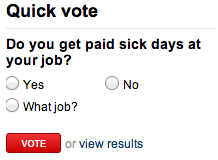
\includegraphics[width=0.25\textwidth]{\chp1@path/1-3_sampling_principles_strategies/figures/vol_resp_bias/vol_resp_bias_q}\pause
		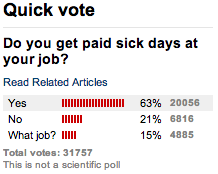
\includegraphics[width=0.25\textwidth]{\chp1@path/1-3_sampling_principles_strategies/figures/vol_resp_bias/vol_resp_bias_res} \\
		{\tiny cnn.com, Jan 14, 2012}
		\end{center}
		\pause
		\item \hl{Convenience sample:} Individuals who are easily accessible are more likely to be included in the sample.

	\end{itemize}

\end{frame}

%%%%%%%%%%%%%%%%%%%%%%%%%%%%%%%%%%%%

\begin{frame}
	\frametitle{Sampling bias example: Landon vs. FDR}

	A historical example of a biased sample yielding misleading results: \\

	$\:$ \\

	\begin{columns}[c]
		\column{0.35\textwidth}
		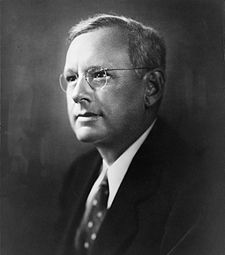
\includegraphics[width= \textwidth]{\chp1@path/1-3_sampling_principles_strategies/figures/landon_fdr/landon}
		\column{0.3\textwidth}
		In 1936, Landon sought the Republican presidential nomination opposing the re-election of FDR.
		\column{0.35\textwidth}
		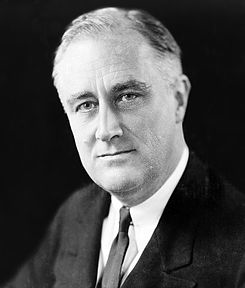
\includegraphics[width= \textwidth]{\chp1@path/1-3_sampling_principles_strategies/figures/landon_fdr/fdr}
	\end{columns}

\end{frame}

%%%%%%%%%%%%%%%%%%%%%%%%%%%%%%%%%%%%%

\begin{frame}
	\frametitle{The Literary Digest Poll}

	\begin{columns}
		\column{0.7\textwidth}

		\begin{itemize}
			\item The Literary Digest polled about 10 million Americans, and got responses from about 2.4 million.
			\item The poll showed that Landon would likely be the overwhelming winner and FDR would get only 43\% of the votes.
			\item Election result:  FDR won, with 62\% of the votes.
		\end{itemize}

		\column{0.3\textwidth}

		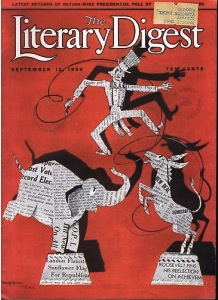
\includegraphics[width= \textwidth]{\chp1@path/1-3_sampling_principles_strategies/figures/literaryDigest}
	\end{columns}

	\begin{itemize}
		\item The magazine was completely discredited because of the poll, and was soon discontinued.
	\end{itemize}

\end{frame}

%%%%%%%%%%%%%%%%%%%%%%%%%%%%%%%%%%%%%

\begin{frame}
	\frametitle{The Literary Digest Poll -- what went wrong?}

	\begin{itemize}
		\item The magazine had surveyed
		\begin{itemize}
			\item its own readers,
			\item registered automobile owners, and
			\item registered telephone users.
		\end{itemize}
		\item These groups had incomes well above the national average of the day (remember, this is Great Depression era) which resulted in lists of voters far more likely to support Republicans than a truly \hl{typical} voter of the time, i.e. the sample was not representative of the American population at the time.
	\end{itemize}

\end{frame}

%%%%%%%%%%%%%%%%%%%%%%%%%%%%%%%%%%%%%

\begin{frame}

	\frametitle{Large samples are preferable, but...}

	\begin{itemize}
		\item The Literary Digest election poll was based on a sample size of 2.4 million, which is huge, but since the sample was \hl{biased}, the sample did not yield an accurate prediction.
		\item Back to the soup analogy: If the soup is not well stirred, it doesn't matter how large a spoon you have, it will still not taste right. If the soup is well stirred, a small spoon will suffice to test the soup.
	\end{itemize}

\end{frame}

%%%%%%%%%%%%%%%%%%%%%%%%%%%%%%%%%%%%%

\subsection{Observational studies}

%%%%%%%%%%%%%%%%%%%%%%%%%%%%%%%%%%%%%

\begin{frame}
	\frametitle{Observational studies}

	\begin{itemize}
		\item Researchers collect data in a way that does not directly interfere with how the data arise.
		\item Results of an observational study can generally be used to establish an association between the explanatory and response variables.
	\end{itemize}

\end{frame}

%%%%%%%%%%%%%%%%%%%%%%%%%%%%%%%%%%%%%

\subsection{Four sampling methods}

%%%%%%%%%%%%%%%%%%%%%%%%%%%%%%%%%%%%%

\begin{frame}
	\frametitle{Obtaining good samples}

	\begin{itemize}
		\item Almost all statistical methods are based on the notion of implied randomness. 
		\item If observational data are not collected in a random framework from a population, these statistical methods -- the estimates and errors associated with the estimates -- are not reliable.
		\item Most commonly used random sampling techniques are \hl{simple}, \hl{stratified}, and \hl{cluster} sampling.
	\end{itemize}

\end{frame}

%%%%%%%%%%%%%%%%%%%%%%%%%%%%%%%%%%%%

\begin{frame}
	\frametitle{Simple random sample}

	Randomly select cases from the population, where there is no implied connection between the points that are selected.

	\begin{center}
	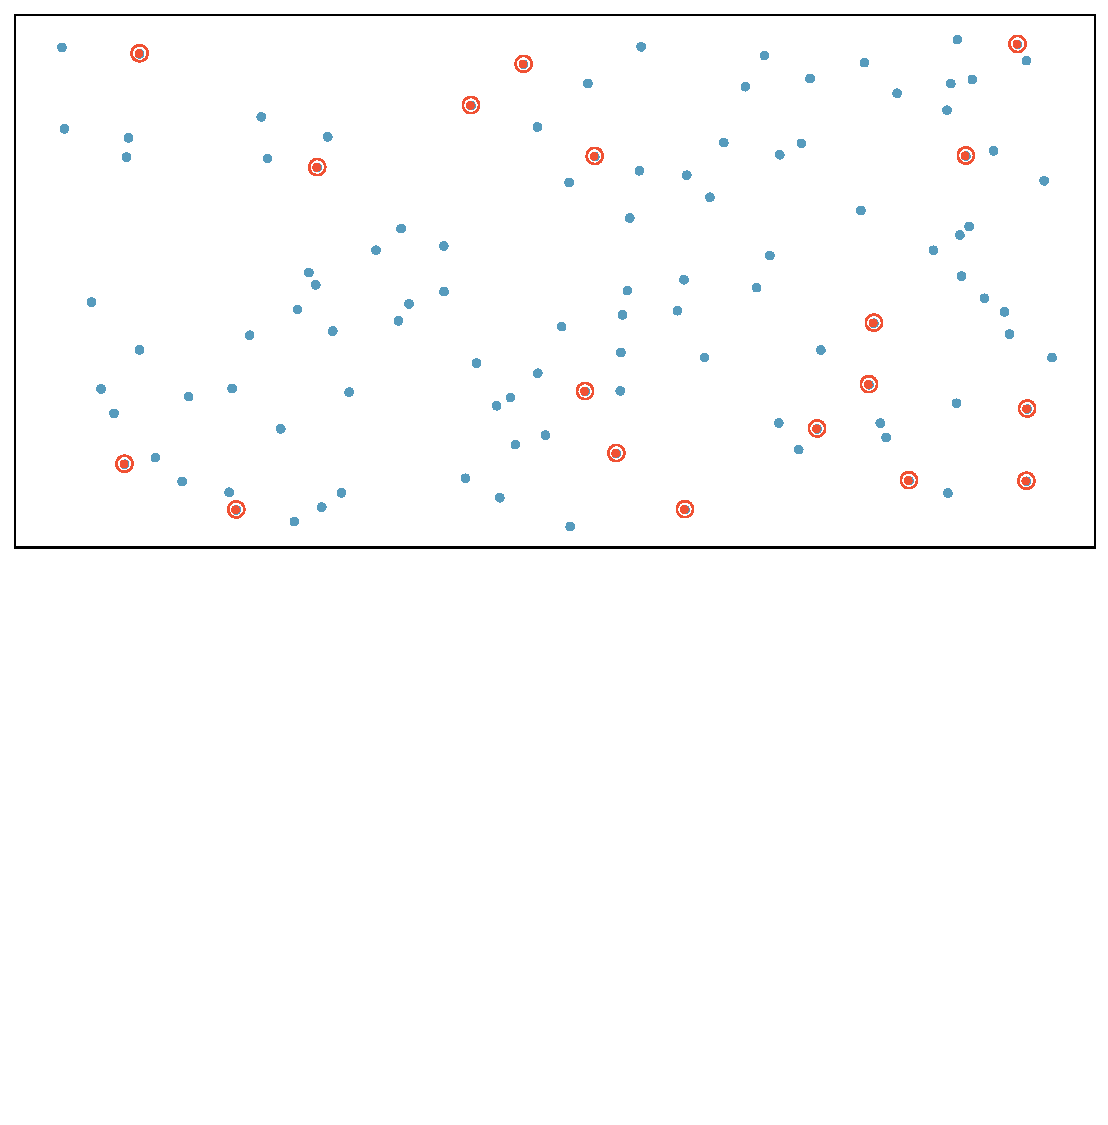
\includegraphics[width=0.9\textwidth]{\chp1@path/1-3_sampling_principles_strategies/figures/sampling_methods/simple}
	\end{center}

\end{frame}

%%%%%%%%%%%%%%%%%%%%%%%%%%%%%%%%%%%%

\begin{frame}
	\frametitle{Stratified sample}

	\hl{Strata} are made up of similar observations. We take a simple random sample from \underline{each} stratum.

	\begin{center}
	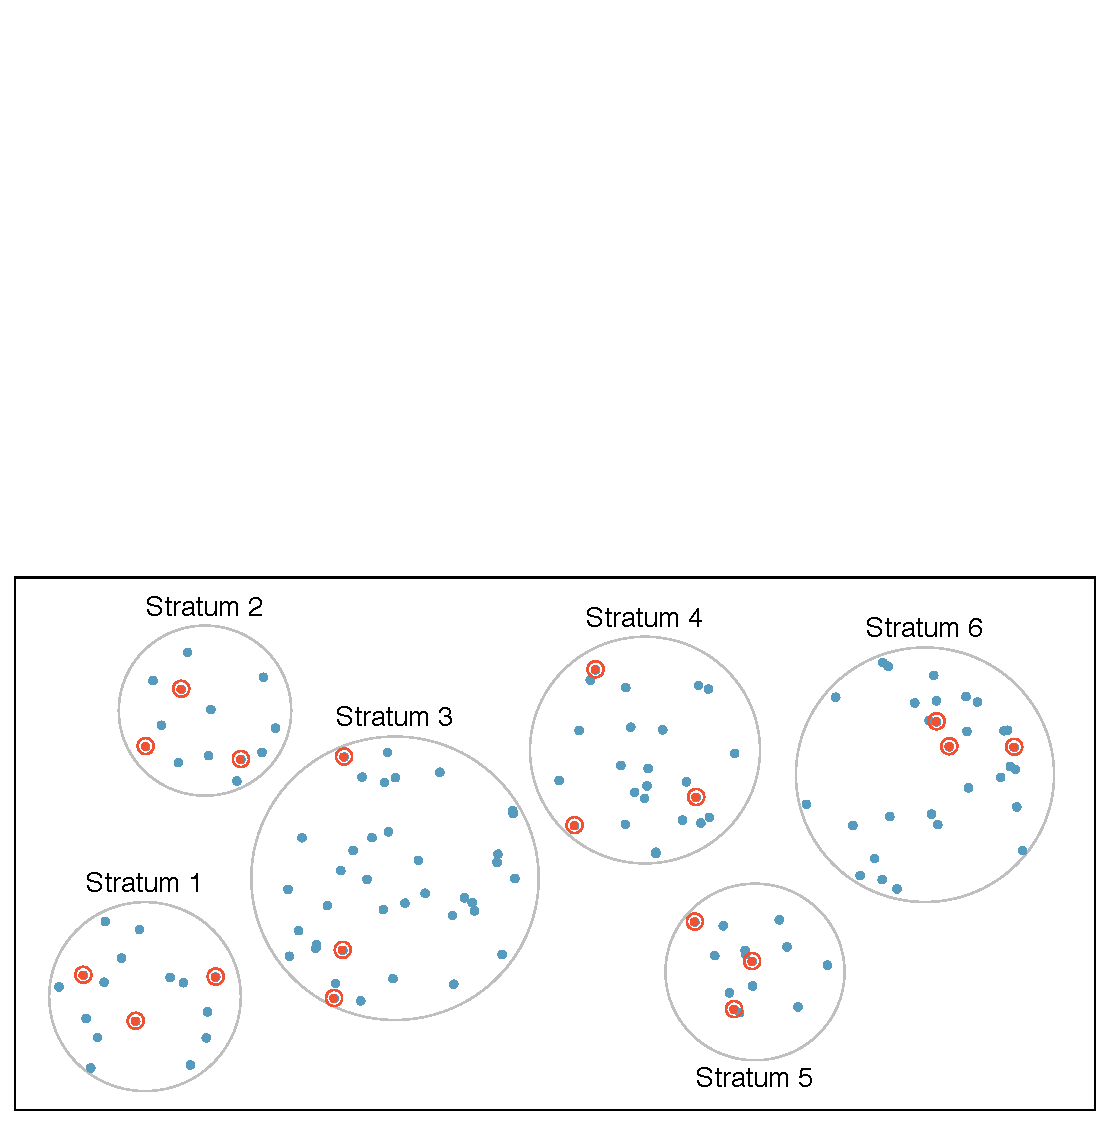
\includegraphics[width=0.9\textwidth]{\chp1@path/1-3_sampling_principles_strategies/figures/sampling_methods/stratified}
	\end{center}

\end{frame}

%%%%%%%%%%%%%%%%%%%%%%%%%%%%%%%%%%%%

\begin{frame}
	\frametitle{Cluster sample}

	\hl{Clusters} are usually not made up of homogeneous observations. We take a simple random sample of clusters, and then sample \underline{all} observations in that cluster. Usually preferred for economical reasons.

	\begin{center}
	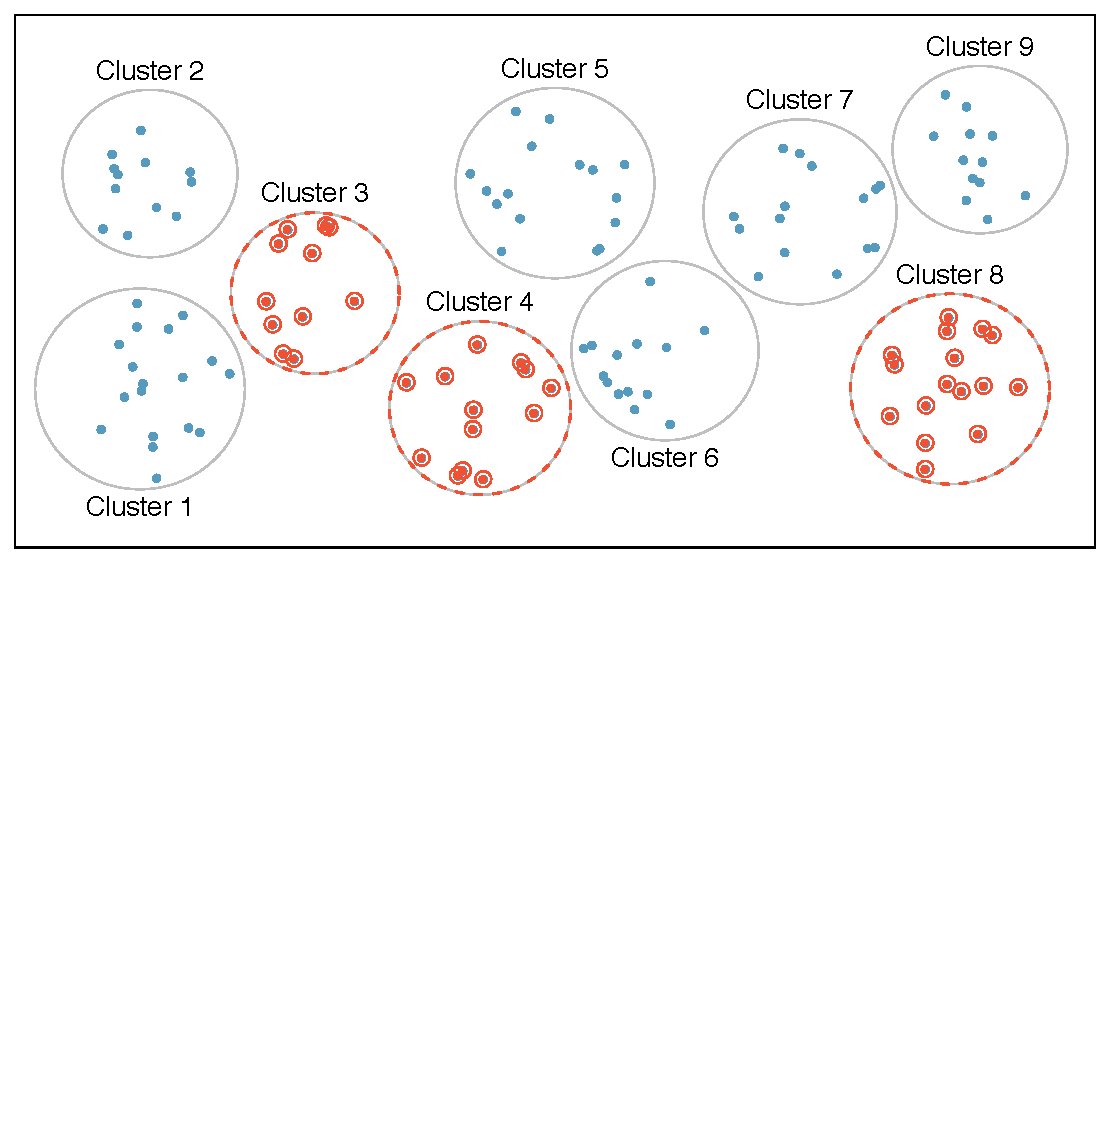
\includegraphics[width=0.9\textwidth]{\chp1@path/1-3_sampling_principles_strategies/figures/sampling_methods/cluster}
	\end{center}

\end{frame}

%%%%%%%%%%%%%%%%%%%%%%%%%%%%%%%%%%%%

\begin{frame}
	\frametitle{Multistage sample}

	\hl{Clusters} are usually not made up of homogeneous observations.  We take a simple random sample of clusters, and then take a simple random sample of observations from the sampled clusters.

	\begin{center}
	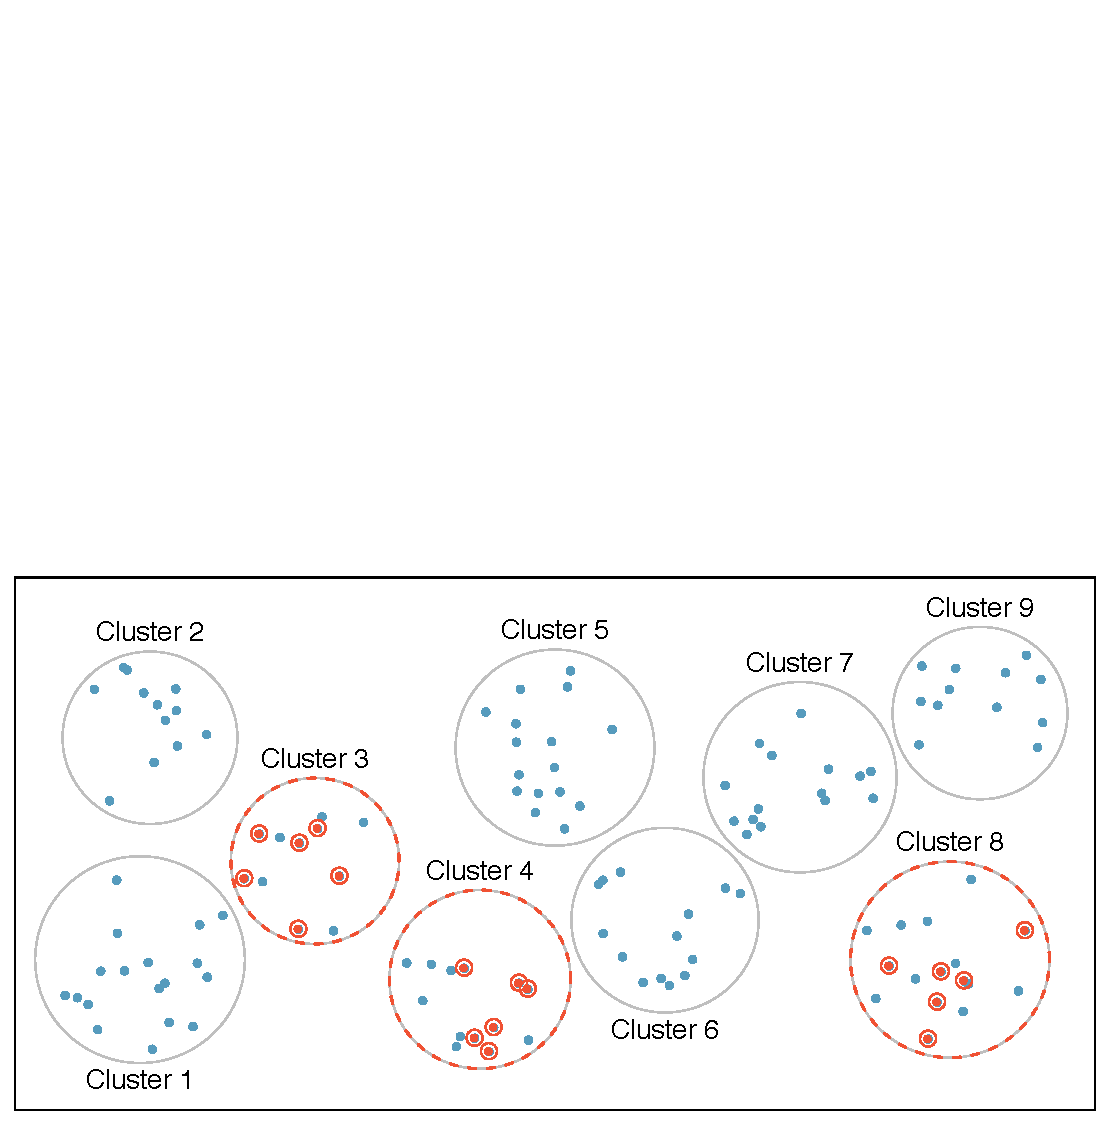
\includegraphics[width=0.9\textwidth]{\chp1@path/1-3_sampling_principles_strategies/figures/sampling_methods/multistage}
	\end{center}

\end{frame}

%%%%%%%%%%%%%%%%%%%%%%%%%%%%%%%%%%%%

%%%%%%%%%%%%%%%%%%%%%%%%%%%%%%%%%%%%
\section{Think/pair/share: sampling/bias}
%%%%%%%%%%%%%%%%%%%%%%%%%%%%%%%%%%%%%

\begin{frame}
	\frametitle{TPS Instructions}

	After reading the question (on the next slide)...

	\begin{itemize}
		\item \textbf{Step 1: Think (3 minute):} Think to yourself about how you would answer the question. You can briefly write down your thoughts for the next steps.
		\item \textbf{Step 2: Pair (2 minutes):} Get into pairs, get to know each other, and discuss the question together. 
		\item \textbf{Step 3: Share (3 minutes):} Share your and your partner's thoughts on the forum, and read others' responses.
	\end{itemize}
\end{frame}

\begin{frame}
	\frametitle{TPS Question}

	A school district purchases language arts software to supplement the teaching of reading to students in grade 2. 
	After 3 months of using the software, the school wants to determine whether use of the program has led to improved reading levels. 
	There is concern that the program may not be as effective for students who are not accustomed to using a computer at home. 
	The district is considering two sampling techniques:

	\begin{enumerate}
		\item Randomly sampling students who have a computer at home and students who don't, and assessing their reading skills. 
		\item Randomly sampling students regardless of whether they have a computer at home or not, and assessing their reading skills. 
	\end{enumerate}

	What is/are the population(s) of interest? Which sampling technique do you think they should use? Why?
\end{frame}

%%%%%%%%%%%%%%%%%%%%%%%%%%%%%%%%%%%%
% End document
%%%%%%%%%%%%%%%%%%%%%%%%%%%%%%%%%%%%

\end{document}